\documentclass[12pt,a4paper]{article} %Formato de plantilla que vamos a usar

\usepackage[utf8]{inputenc}
\usepackage[spanish]{babel}
\usepackage{graphicx}
\usepackage[hidelinks]{hyperref}
\usepackage[table,xcdraw]{xcolor}
\usepackage[margin=2cm,top=2cm,bottom =2.5cm, includefoot]{geometry}
\usepackage{fancyhdr}
\usepackage{listingsutf8}

%Variables
\newcommand{\materia}{SISTEMAS OPERATIVOS Y REDES 2021}
\newcommand{\Date}{12 de Abril de 2021}
\newcommand{\logofacu}{logo-unlp.png}
\newcommand{\unlp}{logo-universidad}
\newcommand{\ing}{logo-ing}

%Definición de colores
\definecolor{colorfacu}{HTML}{4373bf}

%Adicionales
\setlength{\headheight}{50px}
\pagestyle{fancy}
\fancyhf{}
\lhead{\includegraphics[width=4cm]{\unlp}}
\rhead{\includegraphics[width=4cm]{\ing}}
\renewcommand{\headrulewidth}{2pt}
\renewcommand{\headrule}{\hbox to\headwidth{\color{colorfacu}\leaders\hrule height \headrulewidth\hfill}}

%Formato para codigo
\definecolor{codegreen}{rgb}{0,0.6,0}
\definecolor{codegray}{rgb}{0.5,0.5,0.5}
\definecolor{codepurple}{rgb}{0.58,0,0.82}
\definecolor{backcolour}{rgb}{0.95,0.95,0.92}

\lstdefinestyle{customc}{
  belowcaptionskip=1\baselineskip,
  breaklines=true,
  frame=single,
  %xleftmargin=\parindent,
  language=C,
  showstringspaces=false,
  basicstyle=\footnotesize\ttfamily,
  keywordstyle=\bfseries\color{green!40!black},
  commentstyle=\itshape\color{purple!40!black},
  identifierstyle=\color{blue},
  stringstyle=\color{orange},
}


\begin{document}
	\cfoot{\thepage}
	\begin{titlepage}
	\centering                 
	\includegraphics[width=0.8\textwidth]{\logofacu}\par\vspace{1cm}
	{\scshape\LARGE \textbf{\materia}}\par\vspace{0.2cm}
	{\Huge\bfseries\textcolor{colorfacu}{TP n°1 G10}}\par\vspace{1cm}
	{\large Moreyra Iñigo, Juan Martín
66664/6}\par\vspace{0.2cm}
	{\large Piccinini Luca 63207/0}\par\vspace{0.2cm}
	{\large Taboada Rodney 58206/5}\par\vspace{0.2cm}
	{\large \Date\par}
	\end{titlepage}
%-------------------------------------------------------------------------------------------------	
	\clearpage
	\tableofcontents
	\clearpage
%---- Inicio de Documento-----------------%
	\section{Introducción}
	En este informe se detallará la resolución del siguiente enunciado. \par
Escriba un script que cree un directorio con el nombre que se pasa como parámetro en la línea de comandos en el directorio que está almacenado en la variable HOME y copie en él, los archivos terminados en .conf que se encuentran el directorio /etc/
Debe cambiar los permisos de los archivos copiados, cuya tercera letra sea una g, impidiendo el acceso total al resto del mundo y al grupo.\par
Luego debe crear un archivo cuyo nombre también se pasa en la línea de comandos, y almacenar en el los primeros 5 archivos en orden de tamaño creciente y los últimos 5 archivos en orden alfabético decreciente.
	\section{Interpretación}
	Lo que se solicita interpretamos que es lo siguiente:
	\begin{itemize}
		\item Debe realizarse un script en bash que reciba dos parámetros de entrada por línea de comandos.
		\item El primer parámetro es el nombre dado al directorio creado en la variable HOME.
		\item El segundo parámetro es el nombre del archivo que contendrá información recopilada más adelante en la resolución del problema. Este archivo, se guarda en el directorio creado anteriormente.
		\item Una vez creado el directorio,  se copian todos los archivos con extensión “.conf” que se encuentran en el directorio /etc/. Para este punto consideramos ignorar el hecho de que el usuario no tendrá los permisos necesarios para copiar todos los archivos que cumplen la condición, por lo que solo se copiarán los archivos con los permisos válidos.
		\item Luego, se cambian los permisos de todos aquellos archivos copiados cuya tercera letra es una “g”, impidiendo acceso total al resto del mundo y al grupo. Para esto, se usa el comando chmod.
		\item En el archivo anteriormente mencionado (cuyo nombre es el segundo parámetro recibido), se escriben: 
		\begin{itemize}
			\item Los primeros 5 archivos del directorio creado en orden creciente de tamaño.
			\item Los últimos 5 archivos del directorio creado en orden alfabético decreciente.
		\end{itemize}
	\end{itemize}
	\clearpage
	\subsection{Pseudocodigo}
	\lstset{inputencoding=utf8/latin1, style = customc}
    \lstinputlisting[language=C]{pseudocodigo.c}
	\section{Permisos en Linux}
	En los sistemas GNU/Linux existe un sistema de permisos, que otorgan a un determinado usuario o conjunto de estos, el permiso de realizar un conjunto de acciones sobre un determinado archivo. Es importante recordar que todo en Linux es un archivo, ya sea un directorio, un módem, un teclado, etcétera, con lo que este sistema de permisos determina los privilegios de los usuarios sobre el conjunto del sistema.\par
	\subsection{Niveles}
	Los permisos se establecen en tres niveles:
	\begin{itemize}
		\item Propietario, que es aquel usuario que crea el archivo sobre el que se gestionan los permisos
		\item Grupos, es un conjunto de usuarios.\par
		\item Otros usuarios o resto del mundo, que, como el nombre indica, se refiere a los demás usuarios que nos son propietario o no pertenecen al grupo.
	\end{itemize}
	\clearpage
	\subsection{Tipos de permisos}
	Sobre un archivo existen tres tipos de permisos:
	\begin{itemize}
		\item Lectura o read(r), permite que el usuario pueda leer el archivo, es decir ver el contenido del archivo
		\item Escritura o write(w), permite que el usuario pueda escribir el archivo, es decir modificar el contenido del mismo
		\item Ejecución, o execute (x): ejecutar el archivo, es decir, en caso de que el archivo sea un programa, “hacerlo correr”.\par 
	\end{itemize}
	\subsection{Trabajo con permisos}
	Para trabajar con permisos en linux, siempre desde la linea de comando de bash, es esencial el uso de los comandos \textit{ls} y \textit{chmod}.
	\subsubsection{ls}
	El nombre ls se corresponde con la palabra en ingles list o en español listado. El programa permite listar los archivos en distintos formatos de visualización. La opción más útil para el manejo de permisos es la visualización en formato largo, la cual corresponde al comando ls -l.  Este comando da: información de permisos, número de enlaces asociados al archivo, usuario, grupo, tamaño y fecha de última modificación, además del nombre. Ejemplo:\par
	\begin{figure}[h]
		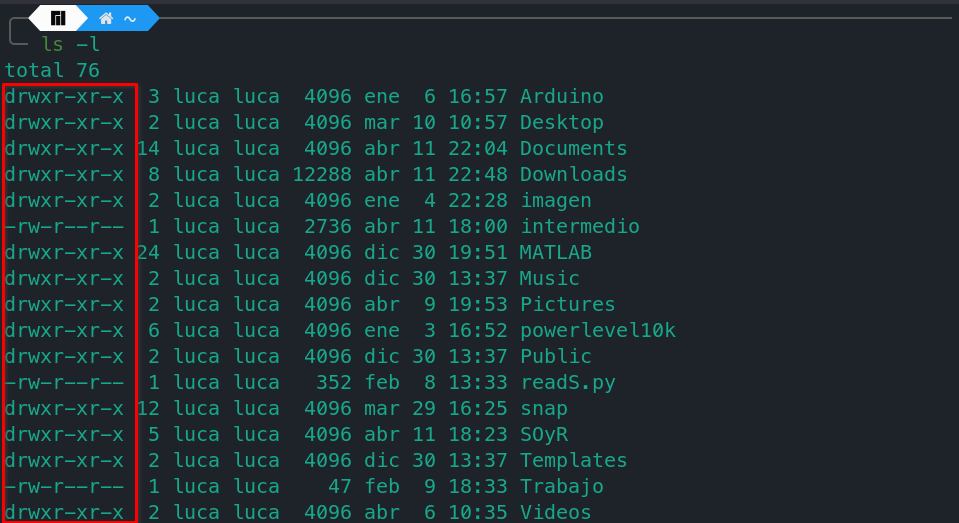
\includegraphics[scale=1]{ls_capture}
		\caption{Captura comando \textit{ls -l} directorio home}
	\end{figure}
	Como vemos el formato de la columna de permisos esta compuesta por 10 posiciones. De izquierda a derecha, la primer posición corresponde al tipo de archivo cuya opciones son:
	\begin{itemize}
		\item - archivo común
		\item d directorio
		\item b archivo de bloques especiales
		\item c archivo de caracteres especiales(Dispositivos tty, impresoras)
		\item l archivo de vinculo o enlace
		\item p archivo especial de cause (pipe o tubería)
	\end{itemize}
	Los siguientes tres caracteres corresponden a los permisos que tiene el propietario, indicado en la tercera columna del comando ls -l, sobre el archivo. Los siguientes tres son los del grupo especificado en la cuarta columna del comando ls -l. Y los últimos tres son los permisos de restos de usuarios. El formato de los tres caracteres para cualquiera de los tres niveles es de la siguiente forma:
	\begin{itemize}
		\item El primer carácter indica si tiene permiso de lectura, este puede estar en \textbf{-} si no tiene este permiso asignado o r si lo tiene asignado.
		\item El segundo carácter indica si tiene permiso de escritura, este puede estar en \textbf{-} si no tiene este permiso asignado o w si lo tiene asignado.
		\item El tercer carácter indica si tiene permiso de ejecución, este puede estar en \textbf{-} si no tiene este permiso asignado o x si lo tiene asignado.
	\end{itemize}
	Veamos un ejemplo, usando la misma captura de la figura 1 podemos extraer la segunda fila\par
	\begin{figure}[h]
		
\includegraphics[scale=1]{archivo_permisos}
		\centering
		\caption{Captura comando \textit{ls -l} archivo especifico}
	\end{figure}
	Con lo cual podemos ver que el archivo Arduino es tipo directorio. Ahora para el directorio Arduino tenemos que, el propietario es el usuario luca y los grupos que tienen permisos asignados, es solo el grupo luca. El propietario tiene permisos de lectura, escritura y ejecución. Por el contrario, el grupo luca y el resto de usuario solo tiene permisos de lectura y ejecución.
	\clearpage
	\subsubsection{chmod}
	Este comando o programa de línea de comando, permite el cambio de los permisos para los tres niveles de estos. Para este comando existen dos modos de uso, el modo carácter y el modo octal. Para el modo carácter debemos indicar a chmod el nivel sobre el que vamos a actuar, el modo en que vamos a modificar los permisos, los permisos a modificar y el archivo. Para esto tenemos las siguiente opciones.\par
	 \begin{itemize}
		\item Indicador de nivel de permiso:\par
		\begin{itemize}
			\item \textbf{u} propietario
			\item \textbf{g} grupo
			\item \textbf{o} otros
			\item \textbf{a} todos
		\end{itemize}		 
		\item Permisos:
		\begin{itemize}
			\item \textbf{r} permiso de lectura
			\item \textbf{w} permiso de escritura
			\item \textbf{x} permiso de ejecución
		\end{itemize}
		\item Operador o modificador:
		\begin{itemize}
			\item \textbf{+} añade un permiso
			\item \textbf{-} quita un permiso
			\item \textbf{=} establece uno o varios permisos
		\end{itemize}
	\end{itemize}
	
	Con esto podemos generar varias sentencias útiles a la hora de gestionar permisos, por ejemplo para añadir permisos de ejecución a todos la sentencia sera \textit{chmod a+x nombredelarchivo}, o podemos quitar permiso de ejecución y escritura al grupo \textit{chmod g-w-x nombredelarchivo}, podemos gestionar a dos niveles o mas a la vez por ejemplo, asignando todos los permisos al propietario y quitandole al grupo y al resto del mundo los de lectura \textit{chmod u=r-w-x, g-r, o-r nombredelarchivo}.\par
	En el modo octal, los permisos se definen como números binarios de tres bits, donde r es el bit más significativo. Por ejemplo \textit{chmod 754 file}.\par
	\begin{center}
		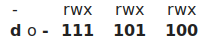
\includegraphics[scale=1]{cuadrito}
	\end{center}
	
	\subsubsection{Un detalle}
	Además de los tres permisos basicos mencionados existen 3 más los cuales no desarrollaremos que son Set User ID(SUID), Set Group ID(SGID) y de persistencia o sticky bit.
\end{document}